\documentclass[aspectratio=169, 11pt]{beamer}
% Department template: Presentation_Report_Guideline_LaTeX_Source, case 1 (research project).
% Numbers are the same as report.tex and come from the result files named in README.md.

\usepackage[utf8]{inputenc}
\usepackage[T1]{fontenc}
\usepackage{helvet}
\renewcommand{\familydefault}{\sfdefault}
\usepackage{xcolor}
\usepackage{booktabs}
\usepackage{graphicx}
\usepackage{amsmath,amssymb}
\usepackage{tikz}
\usetikzlibrary{calc, positioning, arrows.meta}

\definecolor{amritaMaroon}{HTML}{A4123F}
\tikzset{box/.style={draw, rounded corners=2pt, minimum height=1.0cm, text width=2.0cm, fill=#1}, box/.default=gray!8}
\usetheme{Madrid}
\usecolortheme[named=amritaMaroon]{structure}
\setbeamertemplate{navigation symbols}{}
\setbeamertemplate{footline}[frame number]

\begin{document}

\begin{frame}
    \begin{tikzpicture}[remember picture,overlay]
        \node[fill=amritaMaroon, text=white, font=\bfseries\footnotesize, anchor=north east, rounded corners=2pt, inner sep=5pt]
        at ($(current page.north east) + (-0.2cm,-0.2cm)$) {Type 1: Research Project};
    \end{tikzpicture}
    \centering
    
\includegraphics[width=2.6cm]{logo.png}
    \vspace{0.05cm}

    {\large \textbf{\textcolor{amritaMaroon}{MOF Graphs and Crystal Morphology:\\ Crystal Shapes of MOFs from the Unit Cell}}} \\
    \vspace{0.05cm}
    {\footnotesize \textbf{23CSE498 -- Project Phase II (External Review)} \quad | \quad \textbf{Team Number: G070}} \\
    \vspace{0.1cm}
    \begin{table}
        \centering
        \scriptsize
        \renewcommand{\arraystretch}{1.0}
        \begin{tabular}{|c|c|l|}
            \hline
            \textbf{S.No} & \textbf{Register Number} & \textbf{Student Name} \\ \hline
            1 & CB.SC.U4CSE23134 & Pasupuleti Meena Radha Krishna \\ \hline
            2 & CB.SC.U4CSE23122 & Kshitij Varma Pinnamaraju \\ \hline
            3 & CB.SC.U4CSE23031 & Keerthi Sree Jonnakuti \\ \hline
            4 & CB.SC.U4CSE23141 & Rohith Abhinav Sai Komal Gullolla \\ \hline
            5 & CB.SC.U4CSE23029 & Isha Sri Prakash \\ \hline
        \end{tabular}
    \end{table}
    {\footnotesize Guide: \textbf{Dr. T. Ramraj}, Assistant Professor (Sl. Gd.), Department of CSE} \\
    {\scriptsize 13 November 2026}
\end{frame}

\begin{frame}{Guide Review \& Submission Approval}
    \framesubtitle{Confirmation of Project Review and Approval from Guide}
    \centering
    \fbox{\begin{minipage}[c][5.2cm]{0.9\textwidth}
        \centering
        \textbf{[Insert Screenshot of Guide Approval Email Here]} \\[0.3cm]
        {\scriptsize To be added by the team after the guide's approval.}
    \end{minipage}}
\end{frame}

\begin{frame}[shrink=8]{1. Problem Definition \& Research Motivation}
    \framesubtitle{Problem Statement, Identified Literature Gap \& Objectives}
    \begin{block}{Problem}
        \footnotesize
        \begin{itemize}
            \item \textbf{Panel's question (Review 1):} ``Is it possible to generate at least a few morphologies from the given unit cell structure?''
            \item \textbf{Why it matters:} a gas enters a crystal through its surface; the shape decides which faces are exposed and how much surface there is per volume.
        \end{itemize}
    \end{block}
    \begin{block}{Literature and gap}
        \footnotesize
        \begin{itemize}
            \item BFDH (geometry), Wulff (energy), Hartman--Perdok (bond chains), CHGNet (learned potential) exist separately.
            \item \textbf{Gap:} no checked route from a MOF's CIF to its allowed faces, its family of shapes, a structure-only prediction scored against many laboratory crystals, and the effect on gas access.
        \end{itemize}
    \end{block}
    \begin{block}{Objectives}
        \footnotesize
        \begin{enumerate}
            \item Allowed faces and shape families from the space group, with proofs.
            \item A favoured shape from geometry and energy, scored against 134 laboratory records with baselines.
            \item Steering and gas-access indicators per shape, with stated limits.
        \end{enumerate}
    \end{block}
\end{frame}

\begin{frame}{2. Proposed Methodology \& Overall Workflow}
    \framesubtitle{From a CIF to a scored crystal shape}
    \centering
    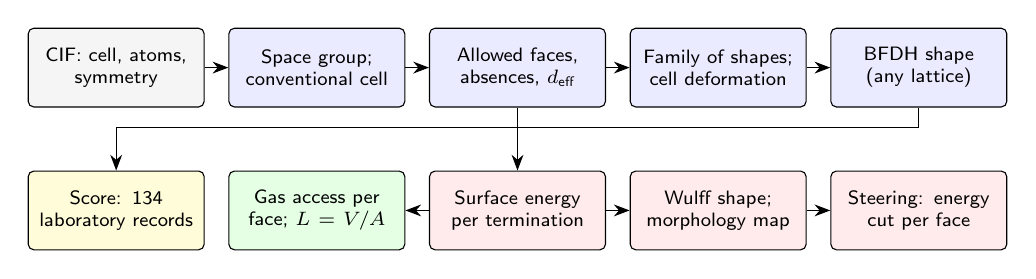
\begin{tikzpicture}[node distance=0.3cm and 0.3cm, every node/.style={font=\scriptsize, align=center}, >={Stealth[length=2mm]}]
    \node[box] (cif) {CIF: cell, atoms, symmetry};
    \node[box=blue!8, right=of cif] (sym) {Space group; conventional cell};
    \node[box=blue!8, right=of sym] (faces) {Allowed faces, absences, $d_\text{eff}$};
    \node[box=blue!8, right=of faces] (fam) {Family of shapes; cell deformation};
    \node[box=blue!8, right=of fam] (bfdh) {BFDH shape (any lattice)};
    \node[box=red!8, below=0.8cm of faces] (gam) {Surface energy per termination};
    \node[box=red!8, right=of gam] (wulff) {Wulff shape; morphology map};
    \node[box=red!8, right=of wulff] (steer) {Steering: energy cut per face};
    \node[box=green!10, left=of gam] (acc) {Gas access per face; $L=V/A$};
    \node[box=yellow!15, left=of acc] (lab) {Score: 134 laboratory records};
    \draw[->] (cif) -- (sym); \draw[->] (sym) -- (faces); \draw[->] (faces) -- (fam); \draw[->] (fam) -- (bfdh);
    \draw[->] (faces) -- (gam); \draw[->] (gam) -- (wulff); \draw[->] (wulff) -- (steer); \draw[->] (gam) -- (acc);
    \draw[->] (bfdh.south) |- ++(0,-0.25) -| (lab.north);
    \end{tikzpicture}
    \vspace{0.3cm}
    \begin{block}{Two independent implementations}
        \footnotesize Python (\texttt{code/morphology/}) and a browser engine (\texttt{website/}), written from the same specification and compared number by number in 15 test suites.
    \end{block}
\end{frame}

\begin{frame}{3. Methodological Components \& Formulation}
    \framesubtitle{Governing equations, dataset and metrics}
    \begin{columns}[T]
        \column{0.5\textwidth}
        \begin{block}{Formulation}
            \scriptsize
            \begin{itemize}
                \item Absent $(hkl)$: $\mathbf{h}R=\mathbf{h}$ and $\mathbf{h}\cdot\mathbf{t}\notin\mathbb{Z}$; $d_\text{eff}=d_{hkl}/n$.
                \item BFDH: face distance $\propto 1/d_\text{eff}$.
                \item $\gamma(s)=\tfrac12 (d/V)\sum \varepsilon_\text{pair}\,c_\text{pair}(s)$; each cut bond 70 kcal/mol; van der Waals 2--7\%.
                \item Cubic map: $x=\gamma_{110}/\gamma_{100}$, $y=\gamma_{111}/\gamma_{100}$; cube $y\ge\sqrt3,\,x\ge\sqrt2$; octahedron $y\le1/\sqrt3$.
                \item Access: probe 1.65 \AA{} (CO$_2$), 1.82 \AA{} (N$_2$); $L=V/A$.
            \end{itemize}
        \end{block}
        \column{0.5\textwidth}
        \begin{block}{Dataset}
            \scriptsize
            \begin{itemize}
                \item 134 records, 35 papers, 12 MOFs: shape, faces, conditions, figure source.
                \item Structures for 8 MOFs; 2 with stand-ins; 138 dataset CIFs for the unvalidated run.
            \end{itemize}
        \end{block}
        \begin{block}{Metrics}
            \scriptsize
            \begin{itemize}
                \item Dominant face and habit against each record.
                \item Baselines: laboratory majority per MOF (paper held out); other MOFs (MOF held out).
                \item Wilson intervals; bootstrap over whole papers.
            \end{itemize}
        \end{block}
    \end{columns}
\end{frame}

\begin{frame}{4. Implementation Details -- Overview}
    \framesubtitle{Module-wise implementation and integration status}
    \begin{table}
        \centering
        \scriptsize
        \renewcommand{\arraystretch}{1.2}
        \begin{tabular}{p{3.2cm} p{8.3cm} c}
            \toprule
            \textbf{Module} & \textbf{Implementation} & \textbf{Status} \\
            \midrule
            Structure and symmetry & CIF reading, symmetry expansion, conventional cell & Integrated \\
            Faces and shapes & Absences, $d_\text{eff}$, BFDH, families, deformed cells, any lattice & Integrated \\
            Energies & Bond-count/UFF cleavage energies; CHGNet slabs (unvalidated) & Integrated \\
            Benchmark, steering, access & Ten MOFs, 134 records; energy cut per face; open fraction per face & Integrated \\
            Website and tests & 27 pages; 15 jsdom suites (over 3\,400 checks); Python tests & Functional \\
            \bottomrule
        \end{tabular}
    \end{table}
    \begin{block}{Environment and repository}
        \footnotesize Python 3.11--3.13 (numpy, scipy, networkx, ase, spglib); JavaScript with three.js; CPU for every result shown; Colab GPU for CHGNet. \texttt{github.com/Radha-Krishna-19/fyp}
    \end{block}
\end{frame}

\begin{frame}{5. Core Module Implementation Details}
    \framesubtitle{The ten-MOF benchmark and the Shape advisor}
    \begin{columns}[T]
        \column{0.5\textwidth}
        \begin{block}{Benchmark (\texttt{run\_benchmark\_mofs.py})}
            \scriptsize
            \begin{itemize}
                \item \textbf{In:} CIF of each MOF; the laboratory CSV.
                \item \textbf{Out:} predicted face and habit; scores per model; MOF-level counts and paper bootstrap.
                \item Primitive cells are converted to the conventional cell first.
            \end{itemize}
        \end{block}
        \begin{block}{Steering and access}
            \scriptsize
            \begin{itemize}
                \item Steering: closed forms for pure shapes; bisection on exact Wulff areas for the dominant face.
                \item Access: plane at the minimum-energy termination, 0.3 \AA{} grid; checked against a 3D estimate.
            \end{itemize}
        \end{block}
        \column{0.5\textwidth}
        \centering
        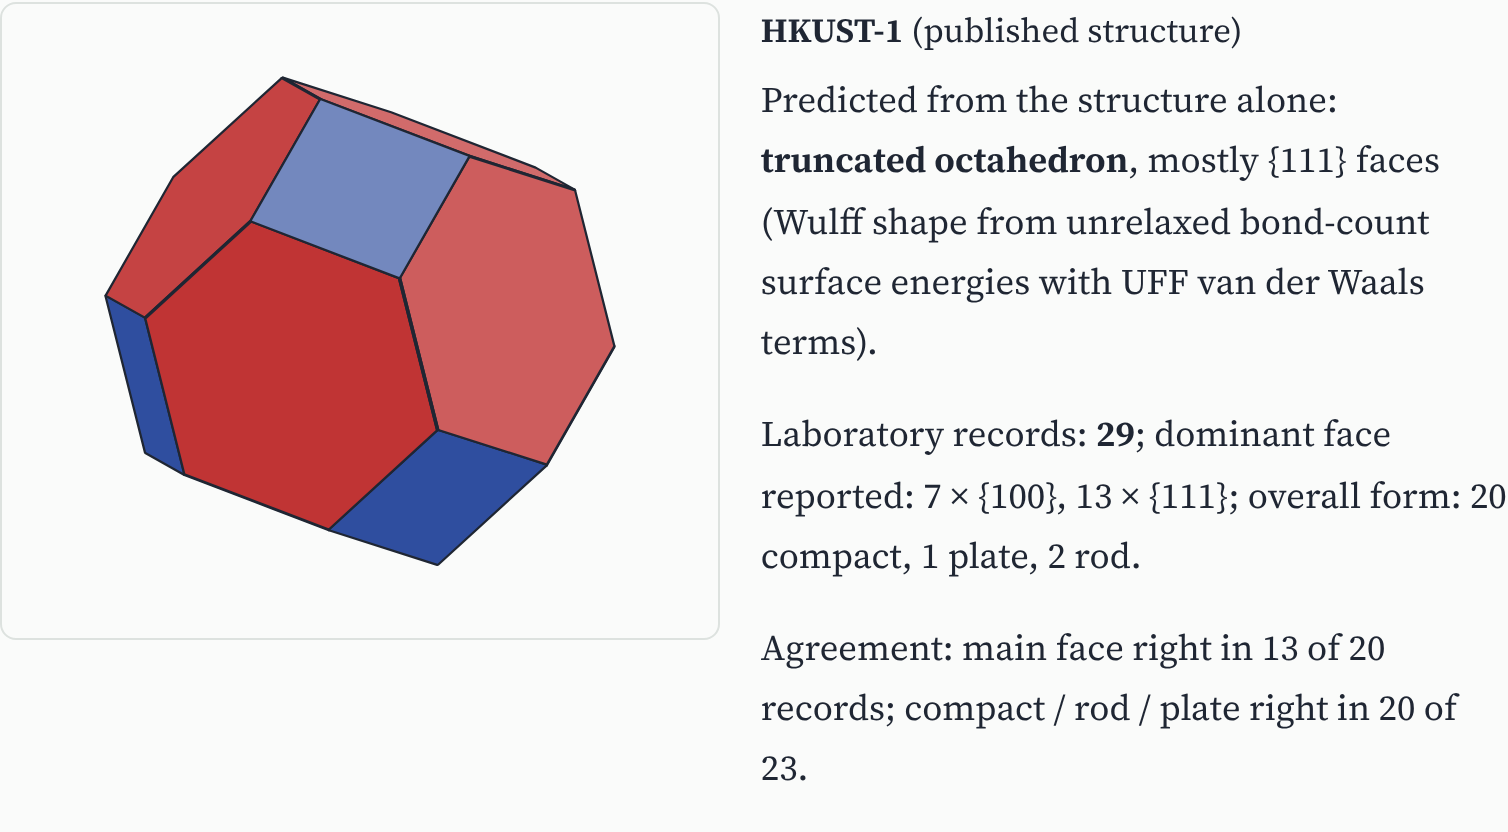
\includegraphics[width=\textwidth]{figures/advisor_hkust1.png}\\
        {\scriptsize Shape advisor page: HKUST-1 predicted shape and laboratory records.}
    \end{columns}
\end{frame}

\begin{frame}[shrink=10]{6. Verification \& Quantitative Results}
    \framesubtitle{Dominant face against laboratory records (eight MOFs with structures)}
    \begin{table}
        \centering
        \footnotesize
        \renewcommand{\arraystretch}{1.15}
        \begin{tabular}{p{5.6cm} c c c}
            \toprule
            \textbf{Model} & \textbf{No additive (32)} & \textbf{With additive (44)} & \textbf{All (76)} \\
            \midrule
            BFDH, structure only & 18 & 21 & 39 \\
            \textbf{Bond-count Wulff, structure only} & \textbf{28} & 17 & 45 \\
            Laboratory majority per MOF, paper held out & 28 & 13 & 41 \\
            Majority of other MOFs, MOF held out & 5 & 17 & 22 \\
            \bottomrule
        \end{tabular}
    \end{table}
    \begin{block}{What this shows, and where it stops}
        \scriptsize
        \begin{itemize}
            \item Without additives: right for \textbf{4 of 5 MOFs} (MOF-5 9/9, ZIF-8 11/12, HKUST-1 7/8, IRMOF-3 1/1; UiO-66 0/2); paper bootstrap 73--97\%. As good as the laboratory majority, with no laboratory data.
            \item With additives no model is reliable. MOFs added after the model was fixed: 1 of 1 without, 1 of 7 with additives.
            \item Habit: 85 of 97 against 76 for ``always compact''; Mg-MOF-74 rods, 9 of 10 crystals elongated.
        \end{itemize}
    \end{block}
\end{frame}

\begin{frame}{7. Visual Results \& Demonstration}
    \framesubtitle{Predicted shapes and the morphology map}
    \begin{columns}[T]
        \column{0.42\textwidth}
        \centering
        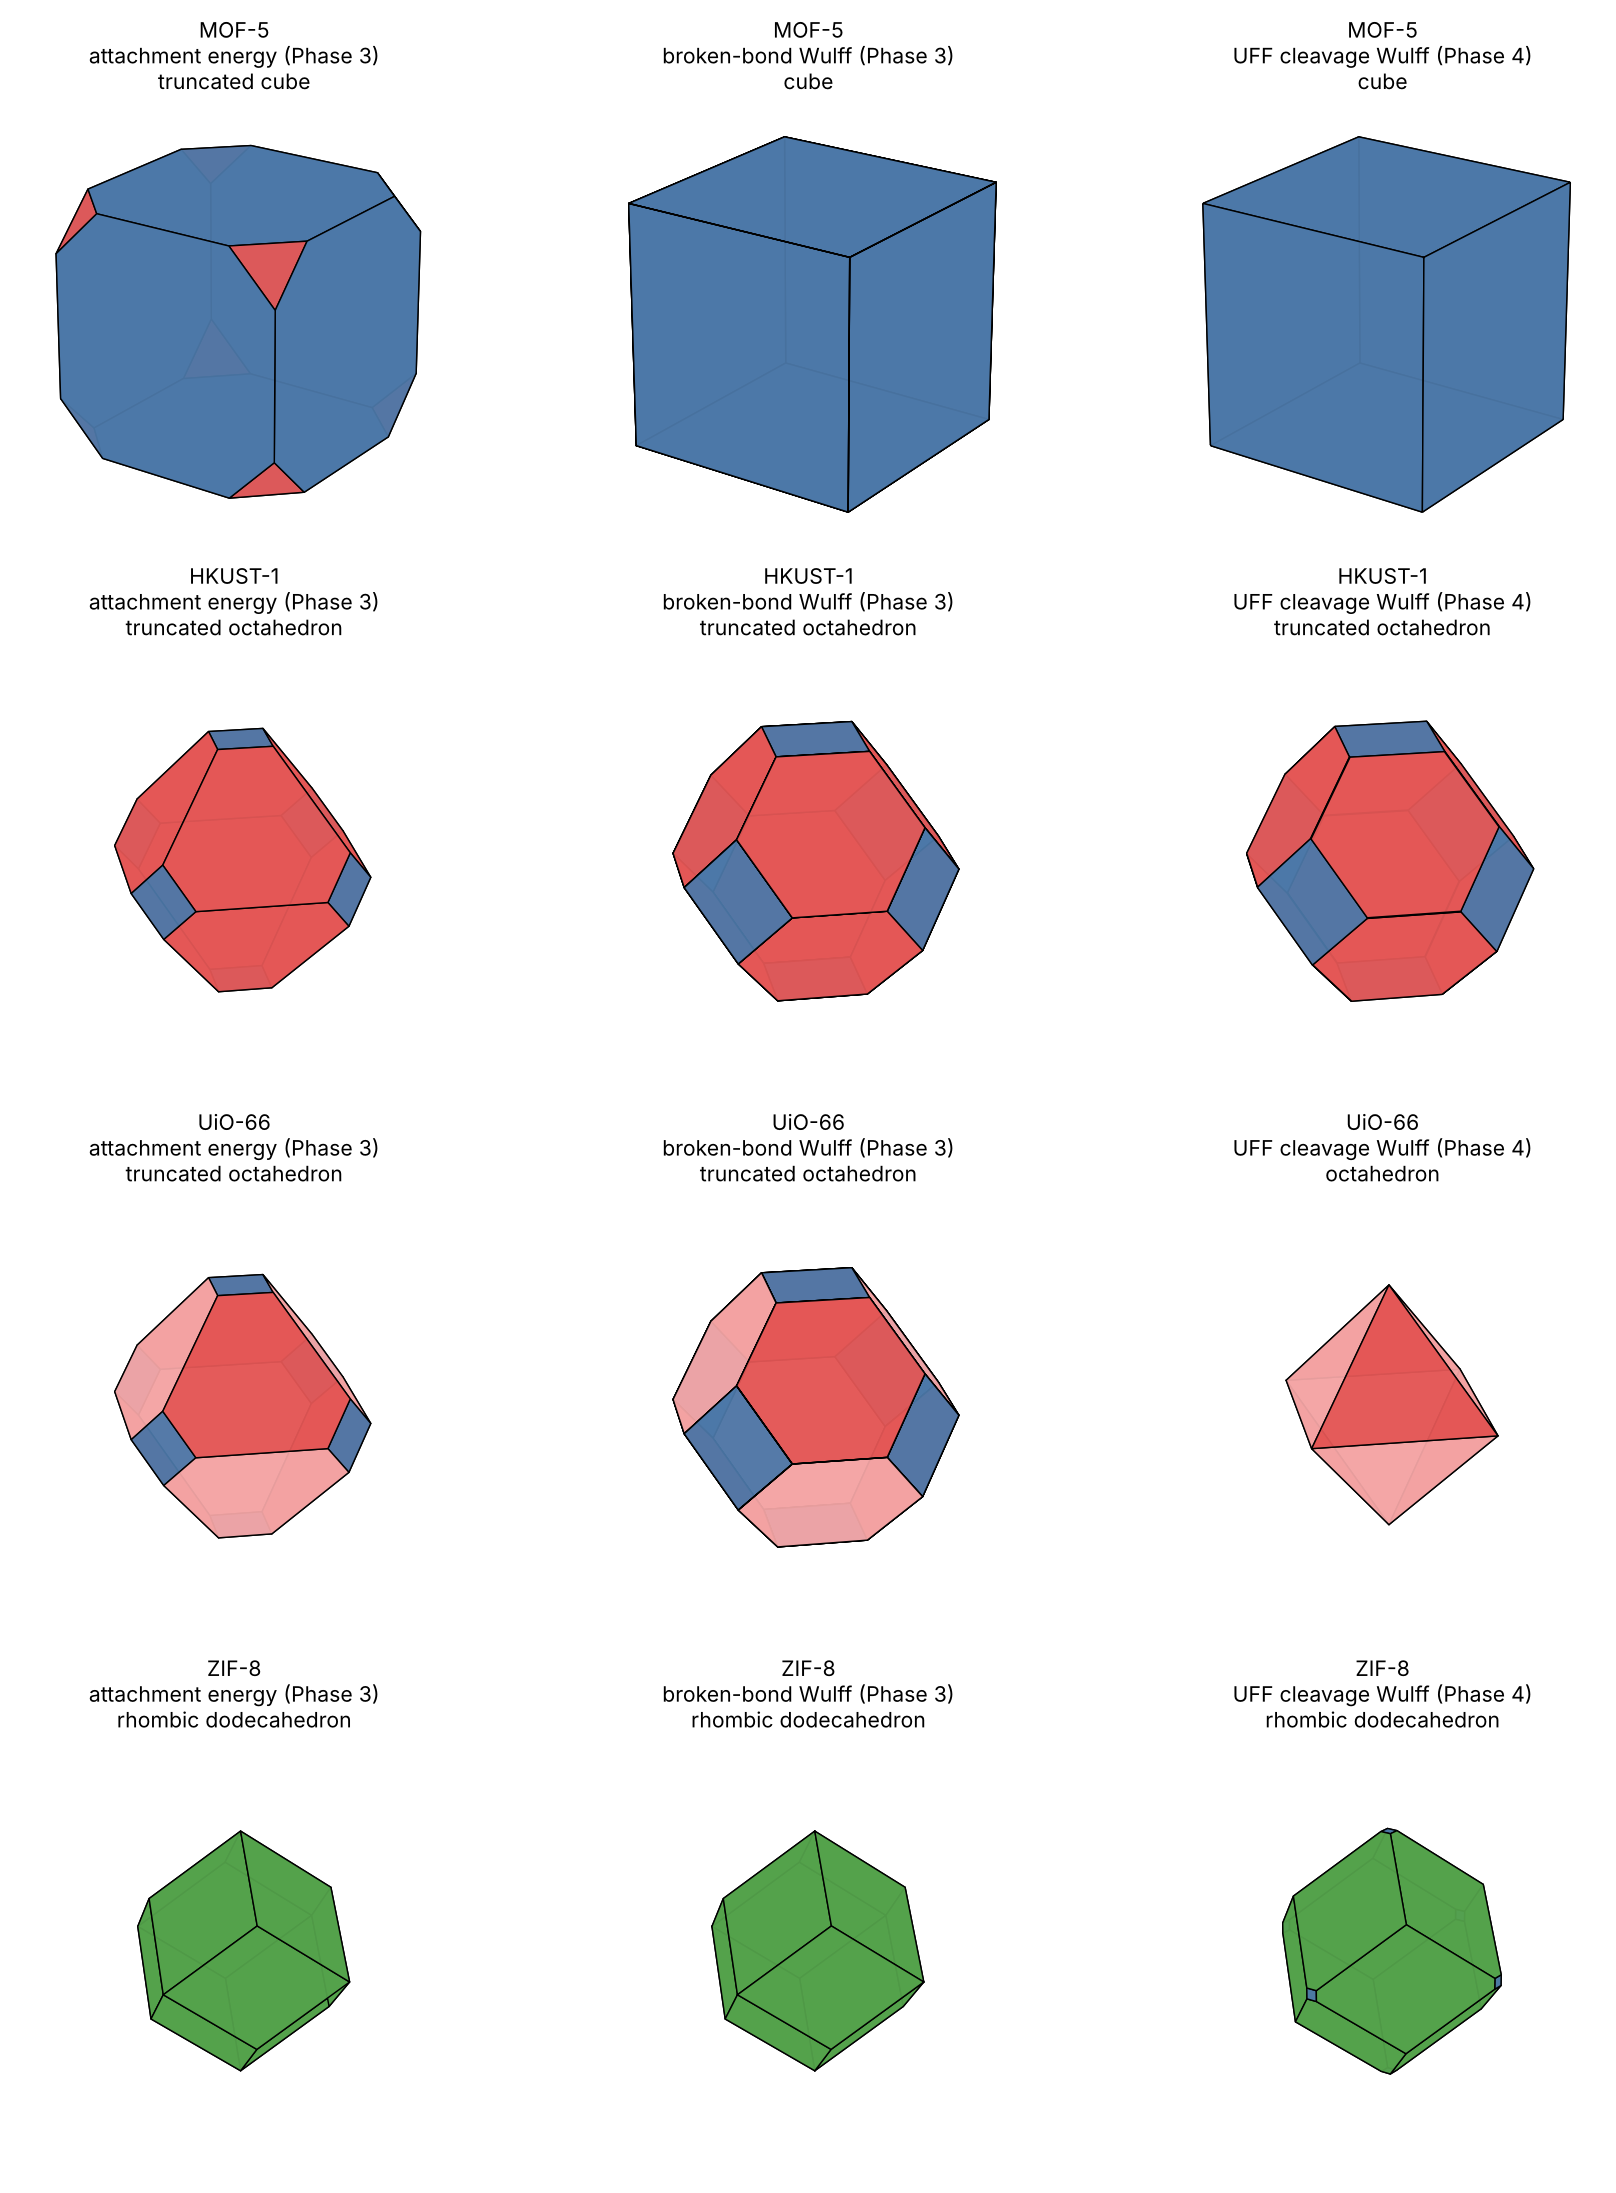
\includegraphics[height=4.6cm]{figures/phase4_compare.png}
        \column{0.56\textwidth}
        \centering
        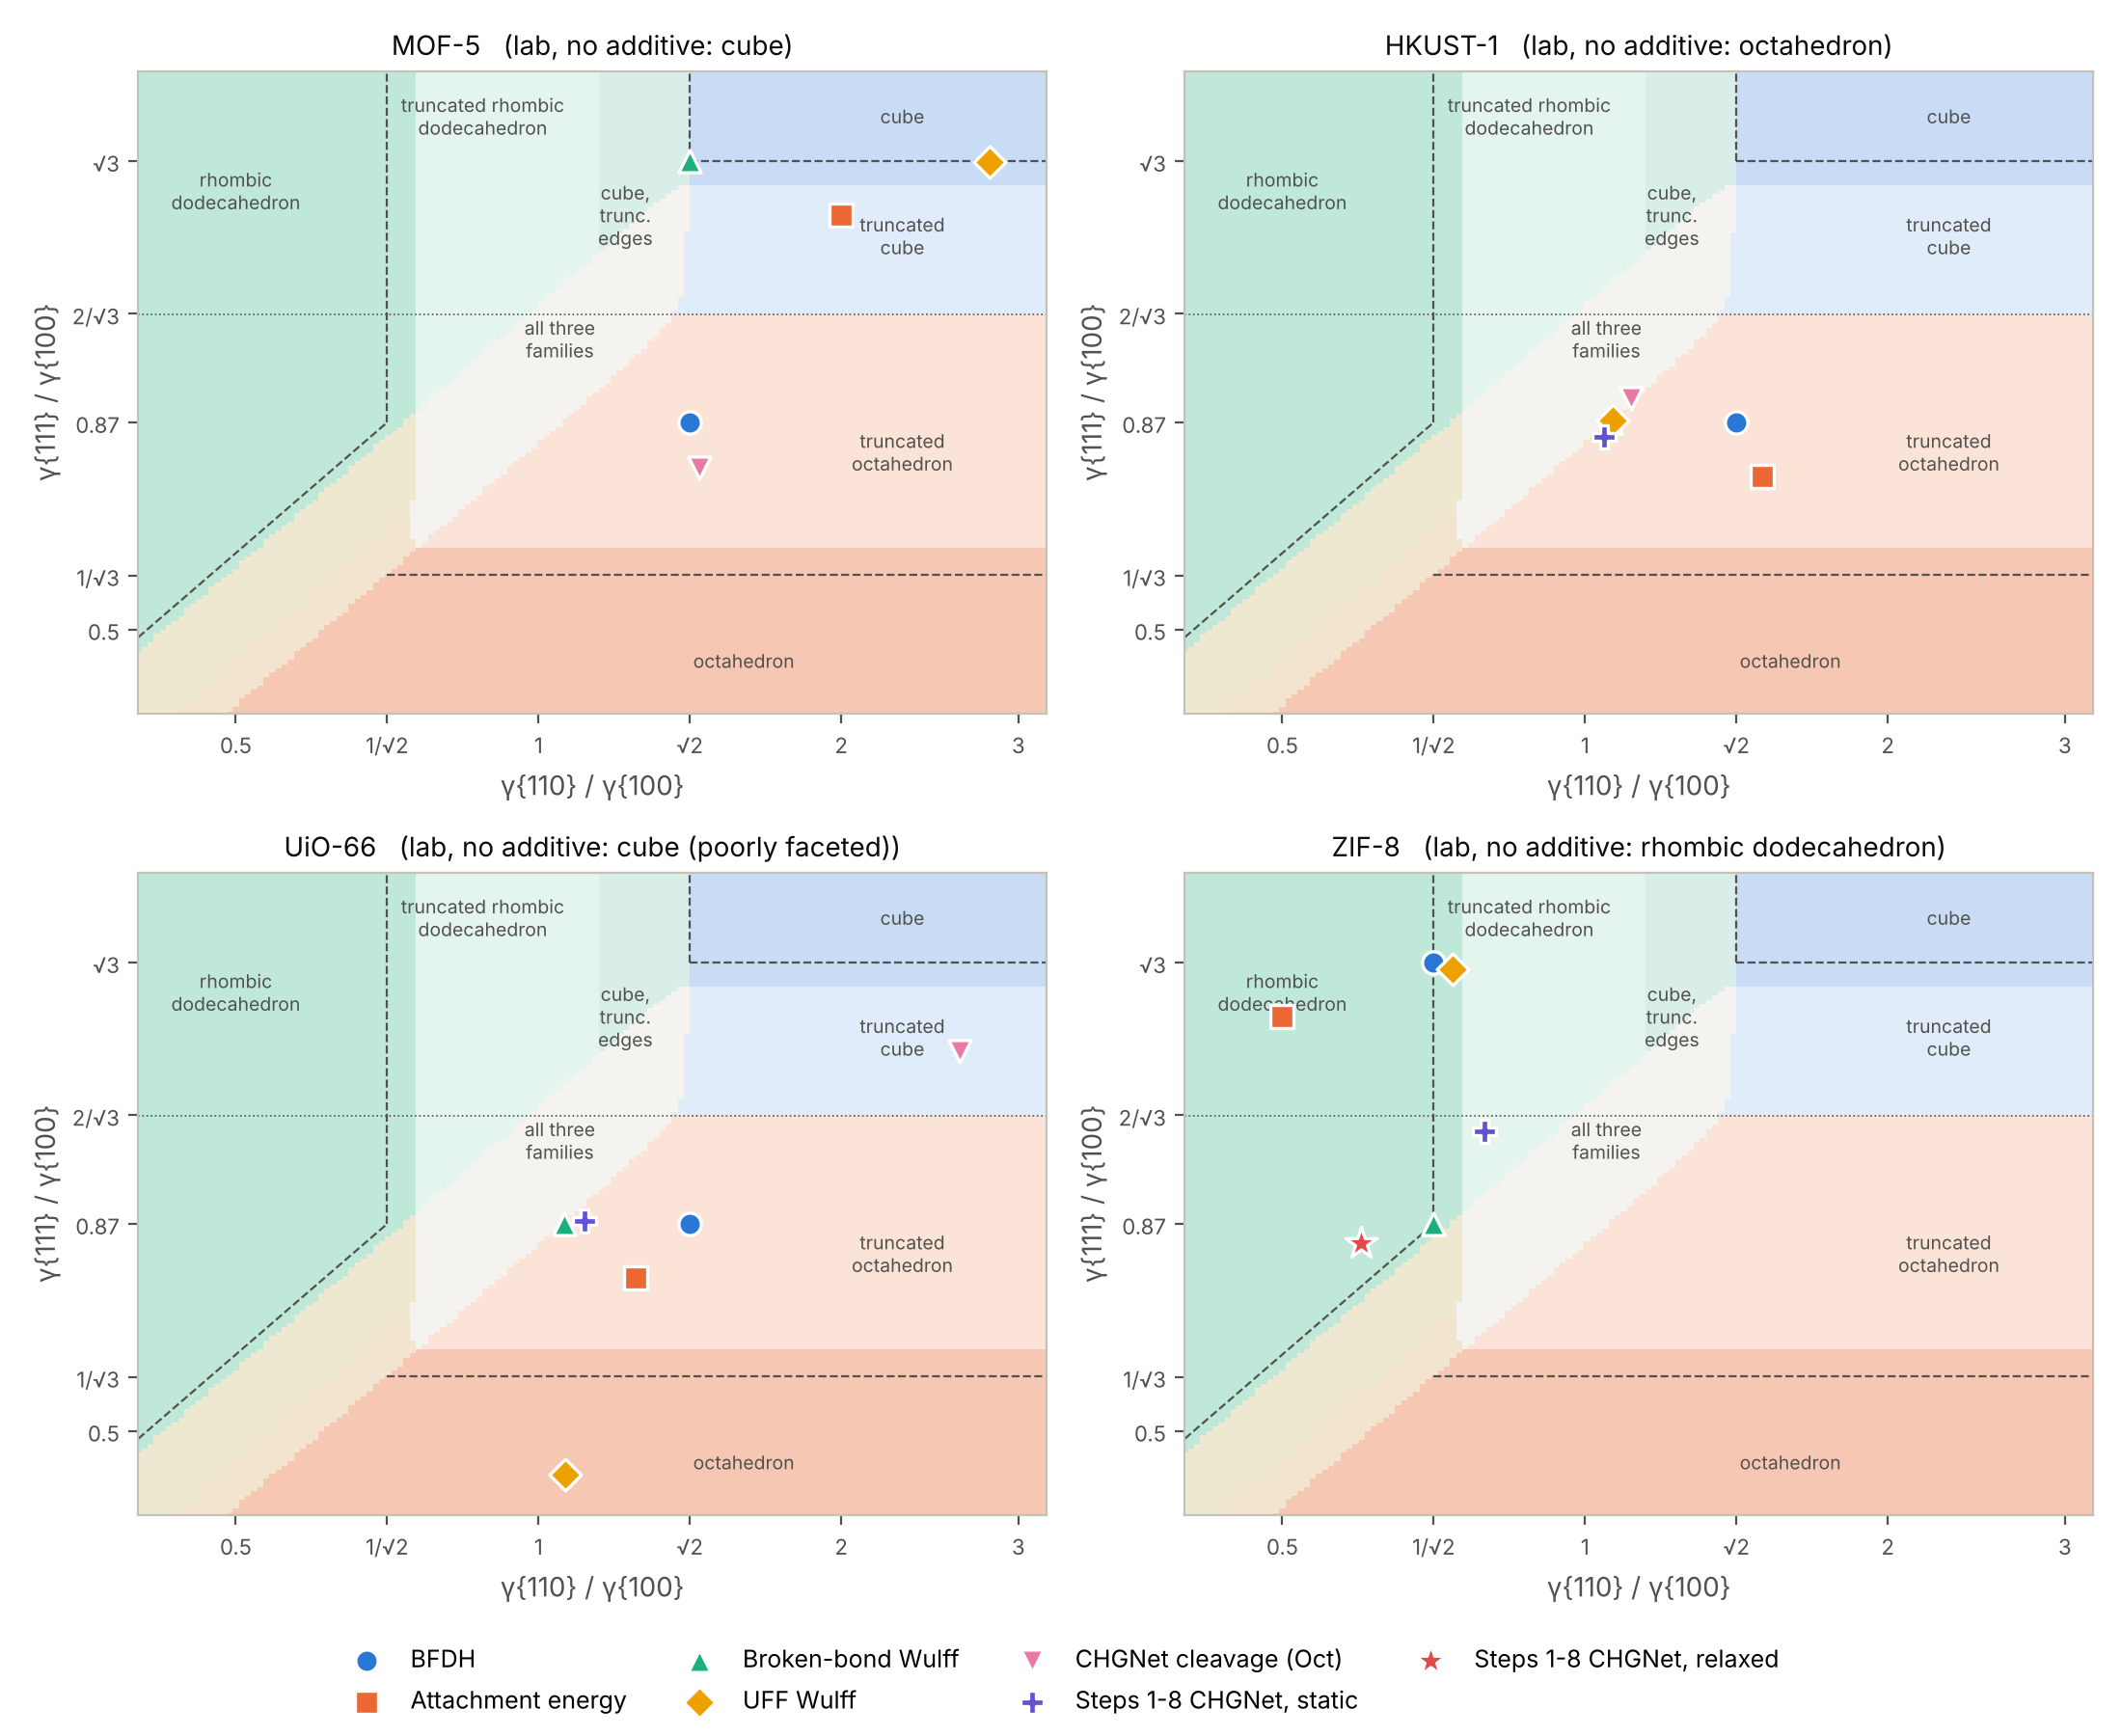
\includegraphics[height=4.6cm]{figures/fig_map_models.png}
    \end{columns}
    \begin{block}{Live demonstration}
        \scriptsize Website: upload a CIF on ``From a CIF to a shape''; choose a MOF on ``Shape advisor'' to see its 3D shape, the energy cut needed for each face, and how open each face is to CO$_2$ and N$_2$.
    \end{block}
\end{frame}

\begin{frame}{8. Technical Justification, Design Trade-offs \& Insights}
    \framesubtitle{Rationale, trade-offs and limits}
    \begin{columns}[T]
        \column{0.48\textwidth}
        \begin{block}{Justification}
            \scriptsize
            \begin{itemize}
                \item BFDH runs on any CIF; the bond-count energy adds what it lacks, with no fitting.
                \item No learned model: shapes exist for 12 MOFs; learning from other MOFs gives 5 of 32.
            \end{itemize}
        \end{block}
        \begin{block}{Trade-offs}
            \scriptsize
            \begin{itemize}
                \item Seconds per MOF, but unrelaxed energies without solvent or electrostatics.
                \item MOF-5's $\gamma_{111}/\gamma_{100}=1.72$ is 0.7\% below $\sqrt3$: its cube rests on one constant.
            \end{itemize}
        \end{block}
        \column{0.48\textwidth}
        \begin{block}{Edge cases}
            \scriptsize
            \begin{itemize}
                \item Primitive cells converted; broken-symmetry files (IRMOF-8, P1 hMOF) flagged.
                \item Unclear additive labels listed; missing faces not scored.
            \end{itemize}
        \end{block}
        \begin{block}{Limitations and future work}
            \scriptsize
            \begin{itemize}
                \item DFT on six prepared slabs; relaxed CHGNet rerun.
                \item Gas access is geometric, not adsorption.
                \item Part I descriptor withdrawn: it follows graph size.
            \end{itemize}
        \end{block}
    \end{columns}
\end{frame}

\nocite{*}
\begin{frame}[allowframebreaks]{References}
    \tiny
    \bibliographystyle{ieeetr}
    \bibliography{ref}
\end{frame}

\begin{frame}
    \centering
    {\Huge \textbf{\textcolor{amritaMaroon}{Thank You}}} \\[0.4cm]
    {\large \textbf{Questions \& Viva Voce}}
\end{frame}

\end{document}
